\section{Heat pump model}

In heat transfer theory the basic thermal circuit contains thermal resistances. Heat transfer occurs via conduction, convection and radiation. In analogy with Ohm's Law for electricity, expressions can be derived for the heat transfer rate (analogous to electrical current) and the thermal resistances (analogous to ohmic resistances) in these three modes of heat transfer. The temperature difference plays a role analogous to the electrical voltage difference. These expressions are shown in Fig. \ref{fig:hpsimulink}.
\begin{figure}[H]
	\centering
	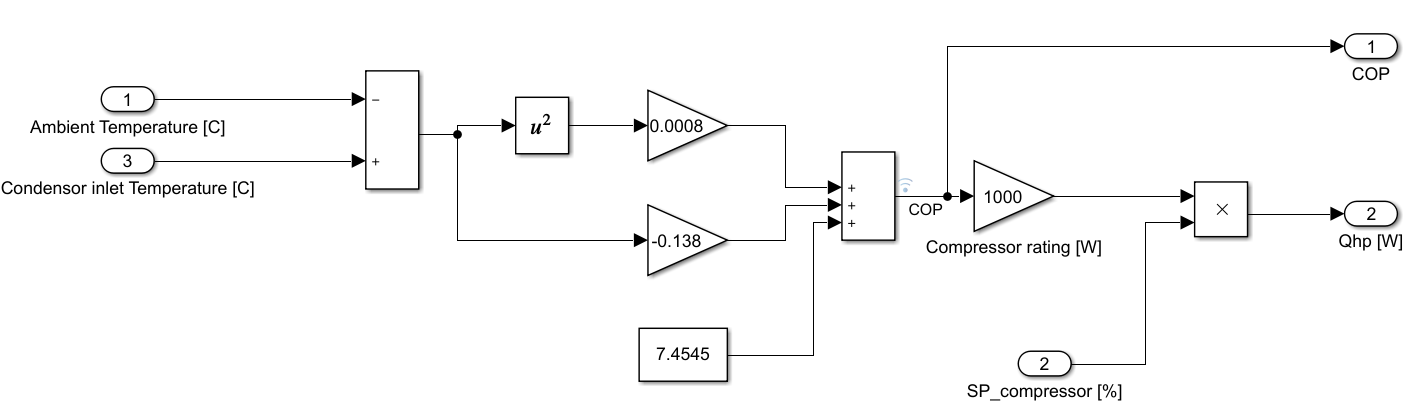
\includegraphics[width=0.8\columnwidth]{Pictures/Heat_Pump.png}
	\caption[Short title]{Heat pump model in Simulink \cite{GIGO}}.
	\label{fig:hpsimulink}
\end{figure}

\lstinputlisting[label=hplist,caption={Heat pump model in Python}, language=Python, linerange={84-88}]{listings/heat_pump.txt}


\begin{figure}[H]
	\centering
	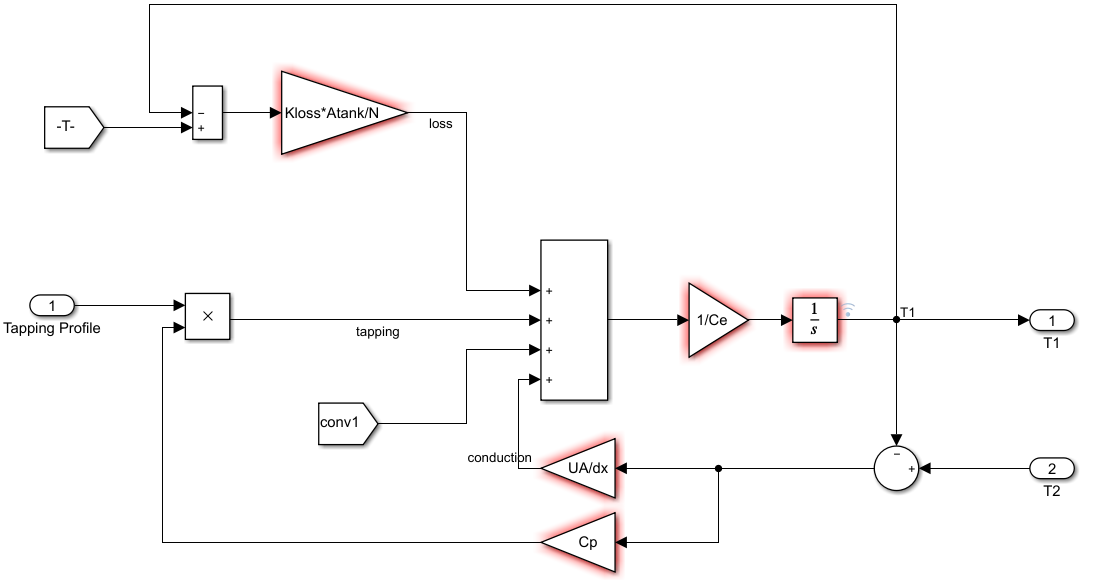
\includegraphics[width=0.8\columnwidth]{Pictures/Layer.png}
	\caption[Short title]{Storage tank layer model in Simulink}.
	\label{fig:layersimulink}
\end{figure}

\begin{figure}[H]
	\centering
	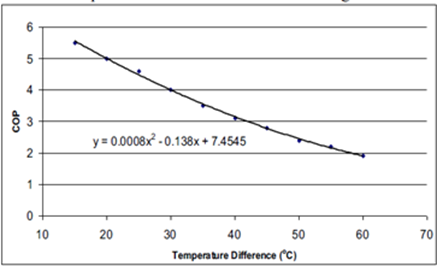
\includegraphics[width=0.8\columnwidth]{Pictures/COPvsDeltaT_Heatpump.png}
	\caption[Short title]{COP vs. Temperature difference between evaporator and condensor side \cite{GIGO}}.
	\label{fig:cop_deltaT}
\end{figure}

Heat transfer rate $\dot{Q}$ in $[W]$

\begin{eqnarray}
	c_{evap} \cdot \frac{dT_{a, out}}{dt} = \dot{m}_{air} \cdot c_{p, air} (T_{a, in} - T_{a, out}) - \dot{Q}_{evap}
\end{eqnarray}

Where $C_{evap} [J/K]$ is the heat capacity of the evaporator. $T_{a,in}$ and $T_{a, out} [K]$ are the temperatures of the air entering and leaving the evaporator, respectively. $\dot{m}_{air} \, [kg/s]$ is the mass flow rate of the air through the evaporator. $\dot{Q}_{evap} [W]$ is the rate of thermal energy delivered by the evaporator.  Note  that  the  last  term $\dot{Q}_{evap}$  can be rewritten as:

\begin{equation}
	\dot{Q}_{evap} = P_{hp} \cdot (COP -1)
\end{equation}

Similarly, from the figure above, the heat balance of the condenser can be written as:

\begin{eqnarray}
	c_{cond} \cdot \frac{dT_{w, out}}{dt} = \dot{m}_{w} \cdot c_{p, w} (T_{w, in} - T_{w, out}) - P_{hp} \cdot COP
\end{eqnarray}

The set of equations presented above characterize the heat delivered by the heat pump as a function of the ambient temperature and the compressor power.

%\newpage
